% Standalone one-pager: HuGaDB GitHub v1 — raw vs cleanup on disk (this repo).
% Build: pdflatex hugadb_github_v1_corpora.tex
% Copy PDF to docs/reports/hugadb_github_v1_corpora.pdf (and optionally results/figures/hugadb/ for figure includes).
\documentclass[11pt]{article}
\usepackage[a4paper,margin=1.8cm]{geometry}
\usepackage[T1]{fontenc}
\usepackage{lmodern}
\usepackage{microtype}
\usepackage{tikz}
\usetikzlibrary{positioning,arrows.meta}
\usepackage{booktabs}
\usepackage{parskip}

\begin{document}
\thispagestyle{empty}

\begin{center}
  {\Large\bfseries HuGaDB GitHub v1 --- two on-disk corpora in this repository}
\end{center}

\vspace{0.5em}
\noindent\small
This project uses the \textbf{official HuGaDB v1} release (GitHub-style filenames \texttt{HuGaDB\_v1\_<activity>\_*.txt}, $\approx$635 trials, 12 activity classes).
There is \textbf{no} internal dataset versioning called ``v2'', ``v3'', or ``v4''; training and loaders read GitHub v1 \texttt{.txt} files from one of two folder layouts below (see \texttt{LoadHuGaDB.m} for the full fallback chain).

\vspace{0.7em}

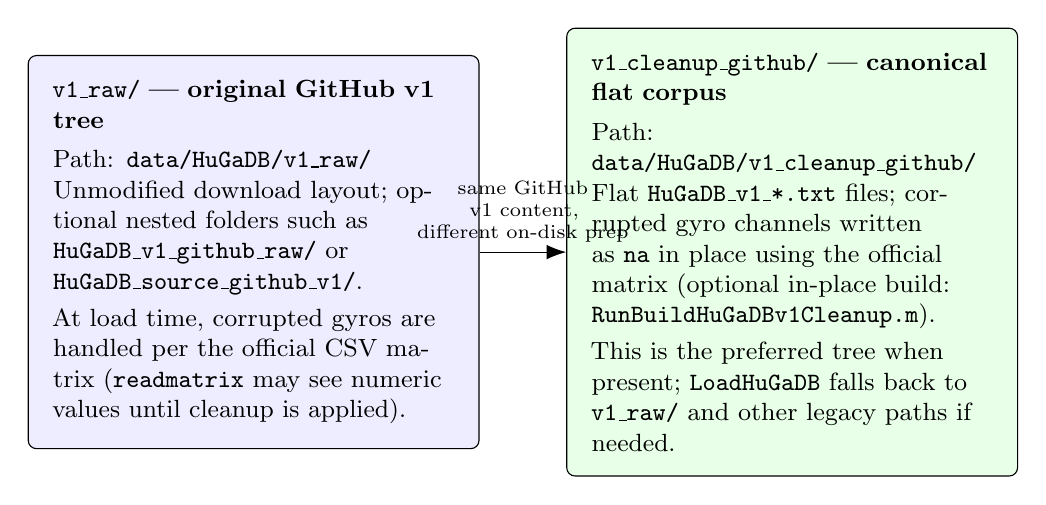
\begin{tikzpicture}[
    node distance=0.5cm and 1.1cm,
    box/.style={draw, rounded corners=3pt, align=left, inner sep=9pt, text width=0.42\textwidth, font=\small}
  ]
  \node[box, fill=blue!7] (raw) {
    \textbf{\texttt{v1\_raw/} --- original GitHub v1 tree}\par\vspace{0.35em}
    Path: \texttt{data/HuGaDB/v1\_raw/}\par
    Unmodified download layout; optional nested folders such as\par
    \texttt{HuGaDB\_v1\_github\_raw/} or \texttt{HuGaDB\_source\_github\_v1/}.\par\vspace{0.25em}
    At load time, corrupted gyros are handled per the official CSV matrix (\texttt{readmatrix} may see numeric values until cleanup is applied).
  };
  \node[box, fill=green!9, right=of raw] (clean) {
    \textbf{\texttt{v1\_cleanup\_github/} --- canonical flat corpus}\par\vspace{0.35em}
    Path: \texttt{data/HuGaDB/v1\_cleanup\_github/}\par
    Flat \texttt{HuGaDB\_v1\_*.txt} files; corrupted gyro channels written as \texttt{na} in place using the official matrix (optional in-place build: \texttt{RunBuildHuGaDBv1Cleanup.m}).\par\vspace{0.25em}
    This is the preferred tree when present; \texttt{LoadHuGaDB} falls back to \texttt{v1\_raw/} and other legacy paths if needed.
  };
  \draw[-{Latex[length=2.5mm]}] (raw.east) -- node[above, font=\scriptsize, text width=2.8cm, align=center] {same GitHub v1 content,\\different on-disk prep} (clean.west);
\end{tikzpicture}

\vspace{0.8em}
\begin{center}
\small
\begin{tabular}{@{}llp{0.52\linewidth}@{}}
  \toprule
  \textbf{Folder} & \textbf{Role} & \textbf{Notes} \\
  \midrule
  \texttt{v1\_raw/} & Original GitHub v1 layout & Not a separate \texttt{v1\_raw\_github/} directory name in this repo. \\
  \texttt{v1\_cleanup\_github/} & Canonical training corpus & Flat files; \texttt{na} gyros where the README matrix marks corruption. \\
  \bottomrule
\end{tabular}
\end{center}

\vspace{0.4em}
\noindent\footnotesize\textit{Implementation:} \texttt{src/acquisition/LoadHuGaDB.m}.

\end{document}
